%% ++++++++++++++++++++++++++++++++++++++++++++++++++++++++++++
%% Anhang: Bilder Nier:Automata
%% ++++++++++++++++++++++++++++++++++++++++++++++++++++++++++++
%
%  Gerüst:
%  * Version 0.11
%  * Skopp, Jonathan, jonathan.skopp@gmail.com
%  * Fachgebiet Kommunikationsnetze, TU Ilmenau
%
%  Für Hauptseminare, Studienarbeiten, Diplomarbeiten, Studium Generale
%
%  Autor           :  Jonathan Skopp
%  Letzte Änderung : 21.05.2019
%

\centering
\chapter{Bilder aus Nier:Automata}

\section{Die Welt}

\restylefloat{figure}

\begin{figure}[h!]
	\centering
	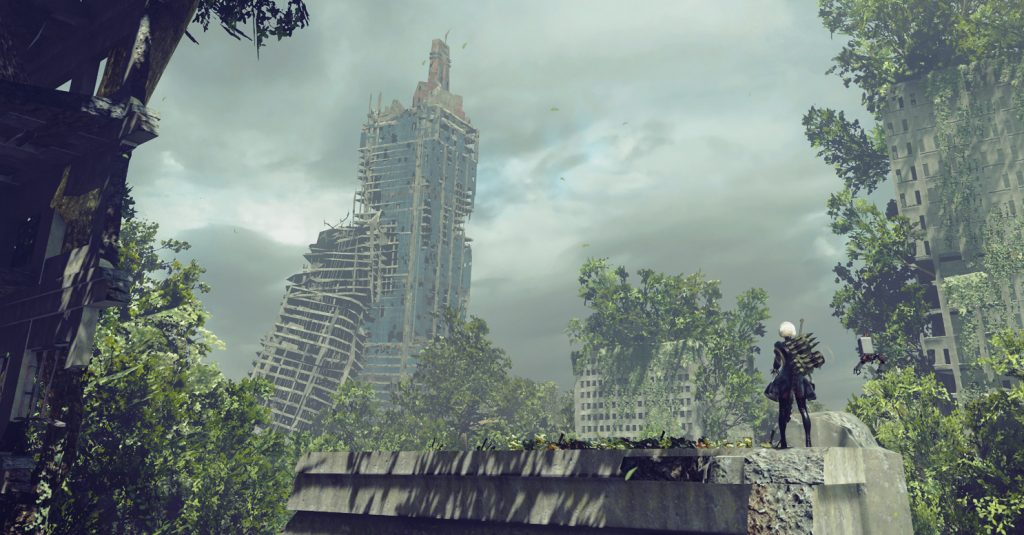
\includegraphics[width=15cm,height=7cm]{Nier/world/area.jpg}
	\caption{Die Ruinenstadt}
	\label{img:passante}
\end{figure}

\begin{figure}[h!]
	\centering
	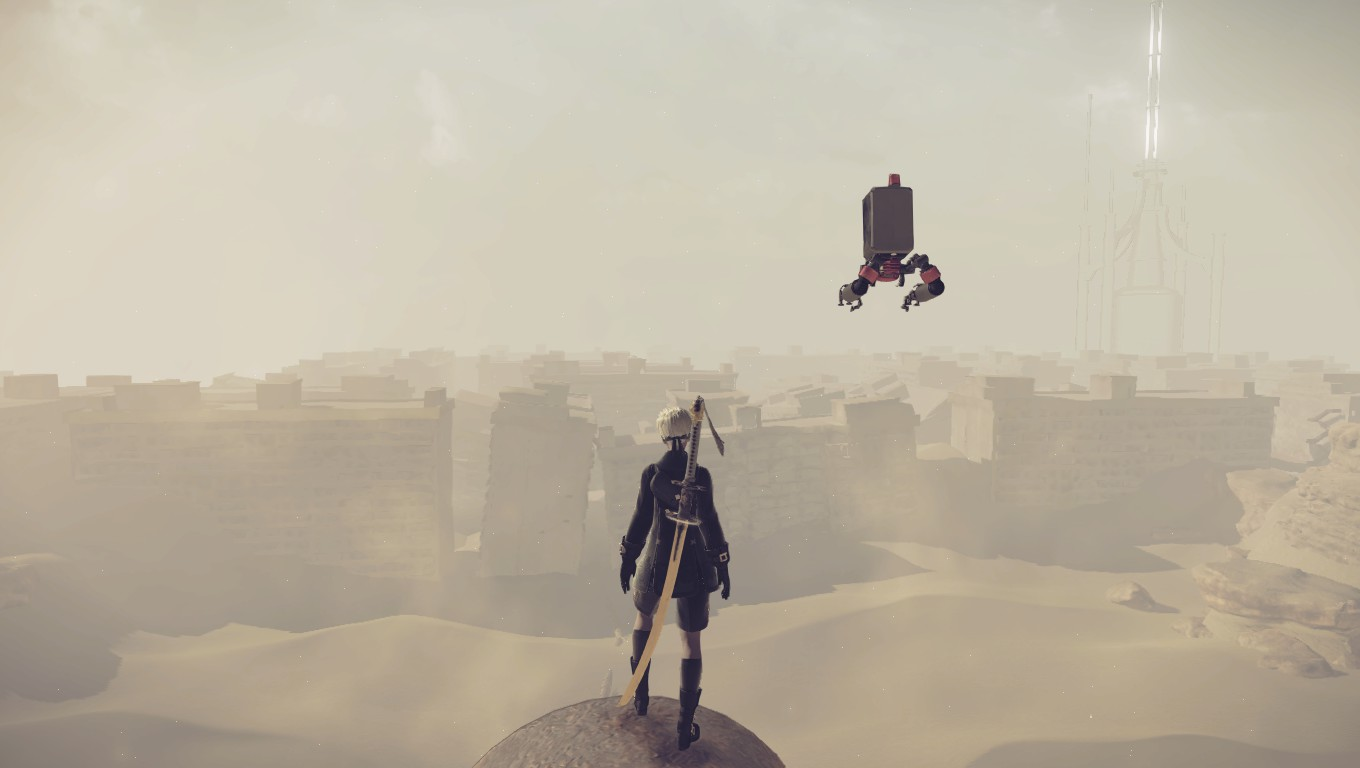
\includegraphics[width=15cm,height=7cm]{Nier/world/desert.jpg}
	\caption{Die Wüste}
	\label{img:passante}
\end{figure}

\begin{figure}[h!]
	\centering
	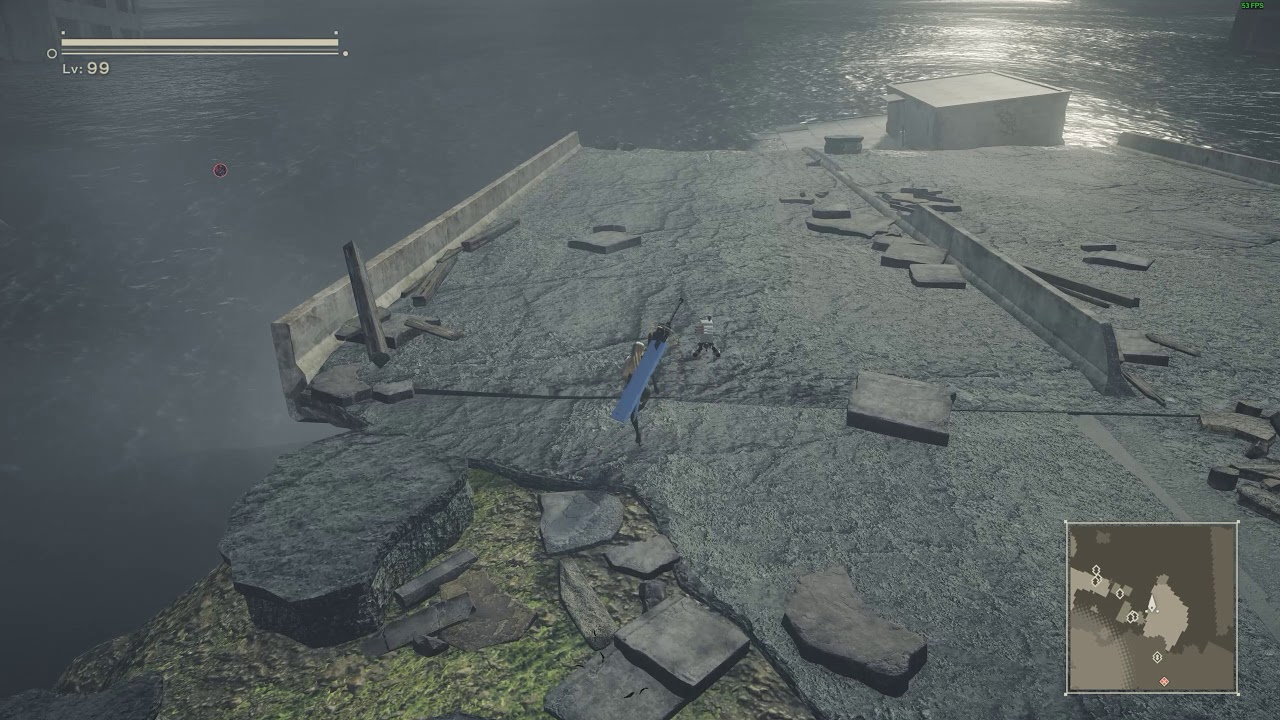
\includegraphics[width=15cm,height=7cm]{Nier/world/water.jpg}
	\caption{Die überflutete Stadt}
	\label{img:passante}
\end{figure}

\begin{figure}[h!]
	\centering
	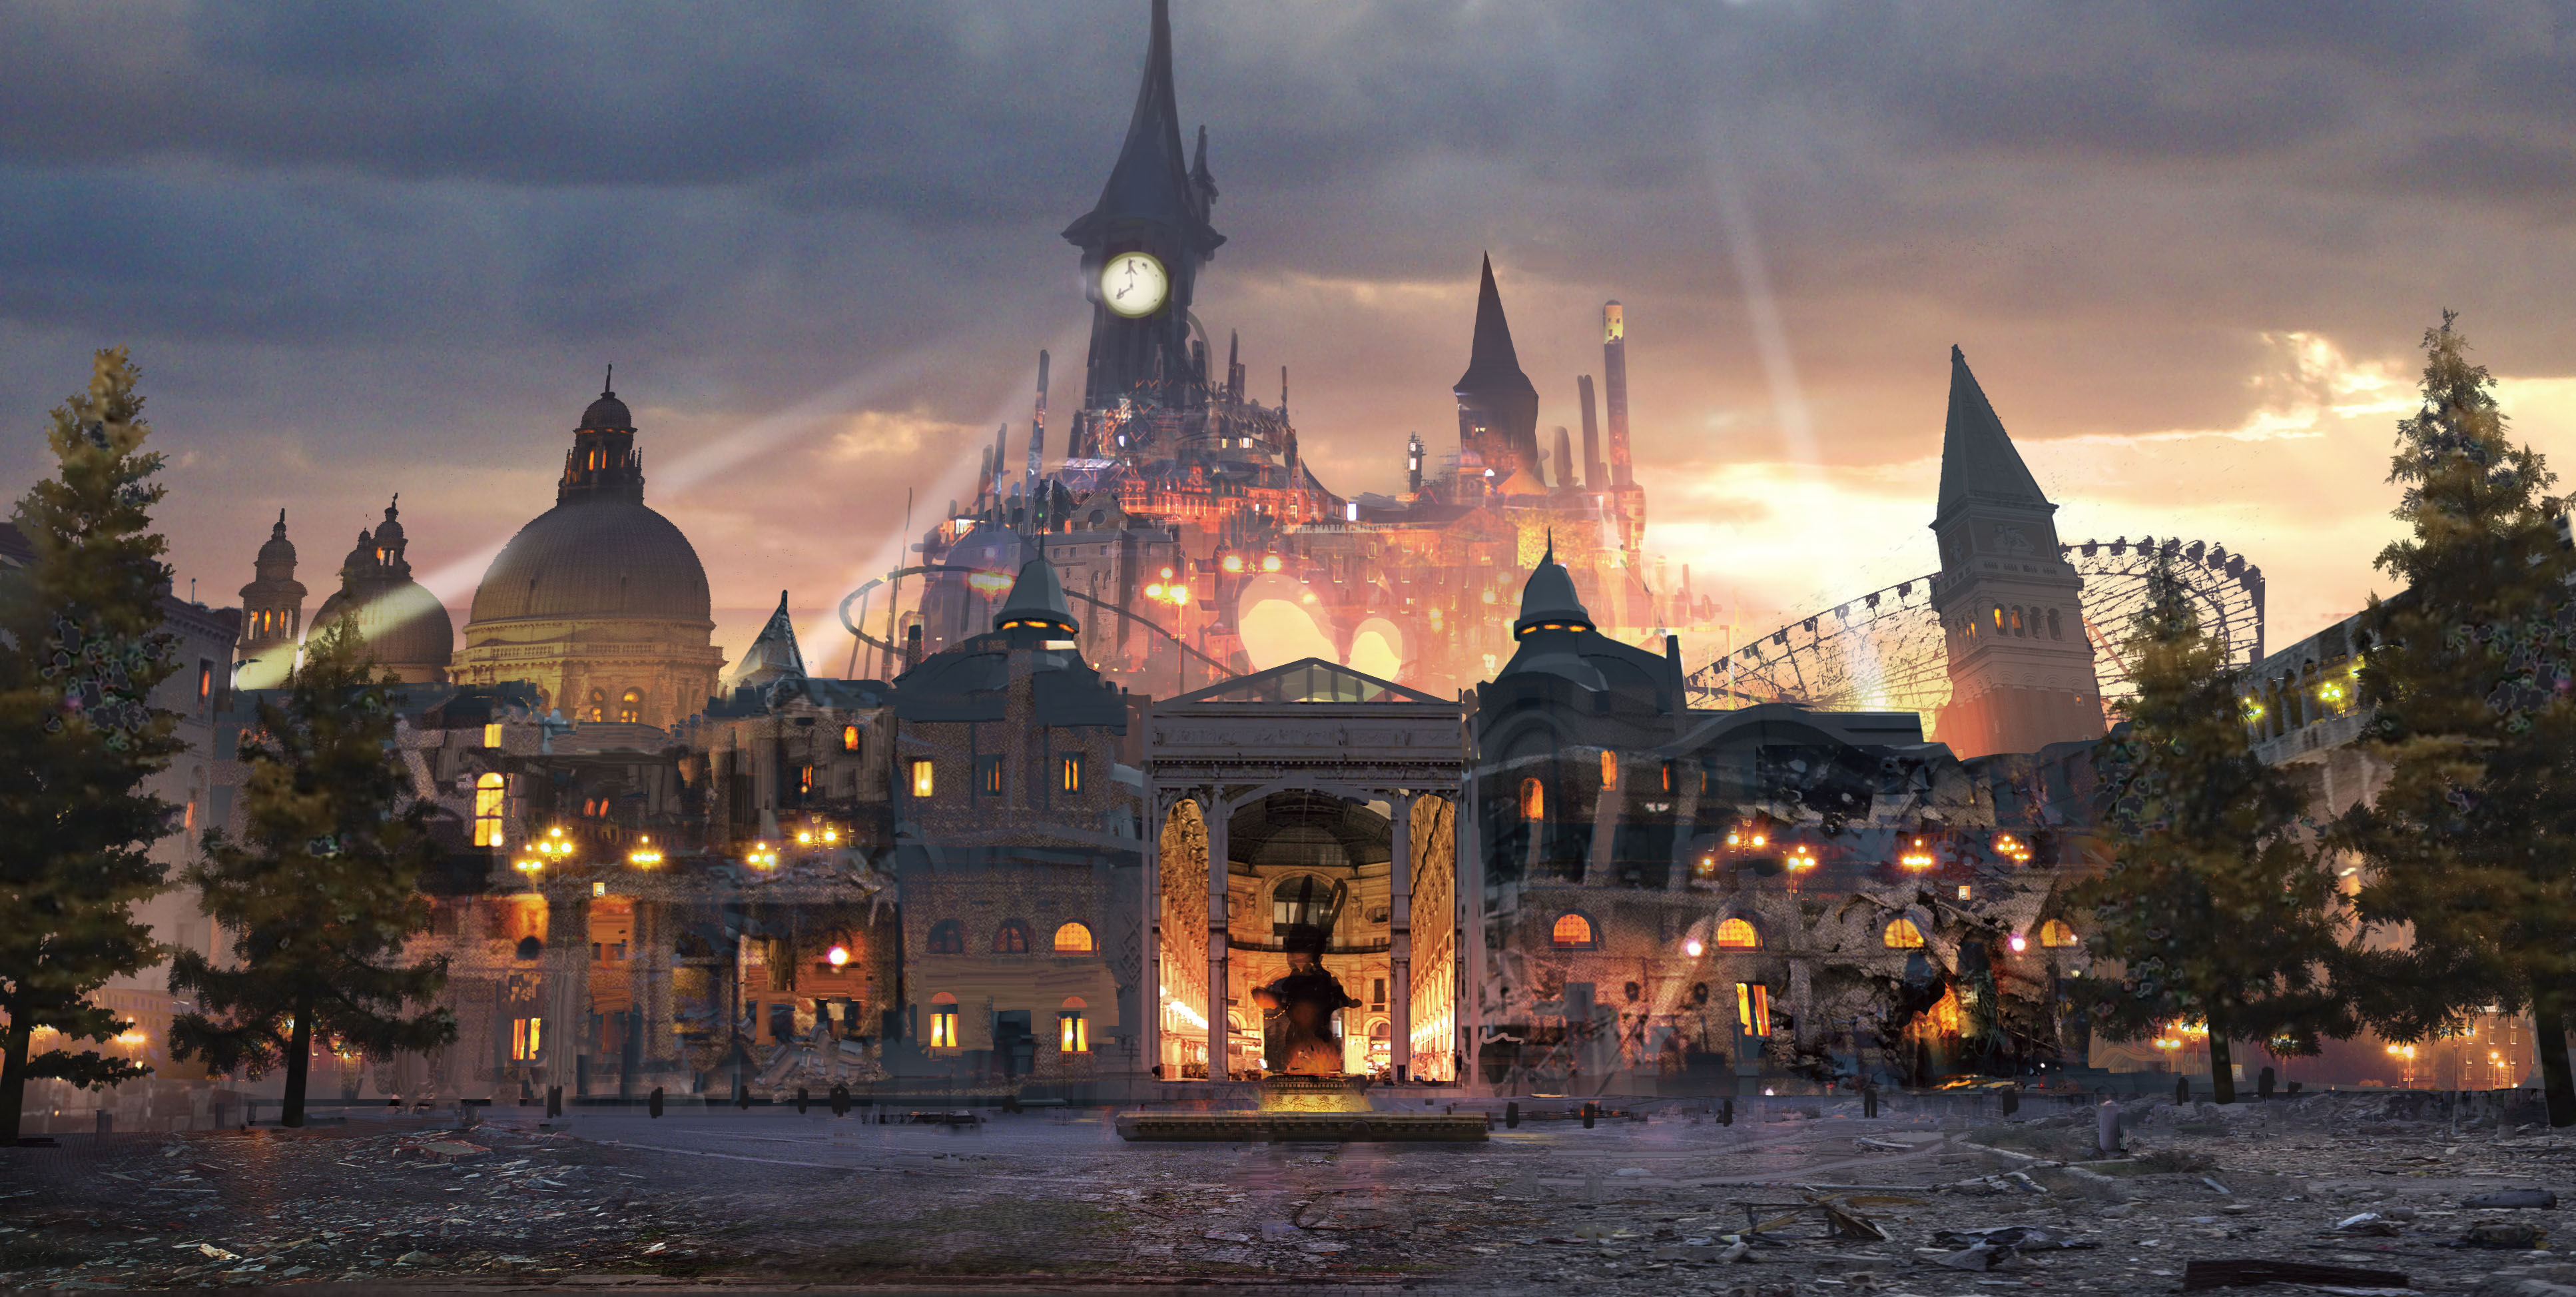
\includegraphics[width=15cm,height=7cm]{Nier/world/fun.jpg}
	\caption{Der Freizeitpark}
	\label{img:passante}
\end{figure}

\clearpage
\section{Die Charaktere}

\begin{figure}[hb!]
	\subfigure[Der humanoide Android 9s]{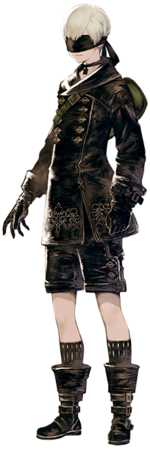
\includegraphics[width=0.49\textwidth,height=17cm]{Nier/Chara/YoRHa_No-9_Type_S.png}} 
	\subfigure[Die humaoide Androidin 2b]{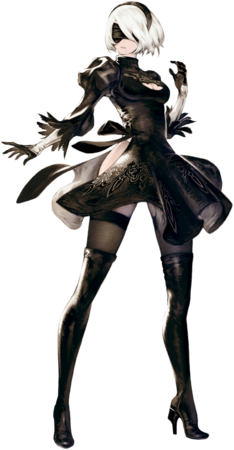
\includegraphics[width=0.49\textwidth,height=17cm]{Nier/Chara/YoRHa_No-2_Type_B.png}} 
	\caption{Die Hauptcharaktere} 
\end{figure}


\clearpage
\section{Wichtige Nebencharaktere}

\begin{figure}[hb!]
	\subfigure[Adam]{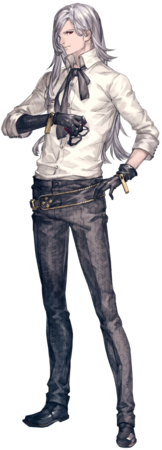
\includegraphics[width=0.49\textwidth,height=17cm]{Nier/Chara/YoRHa_Commander.png}} 
	\subfigure[Die humanoide Androidin 2a]{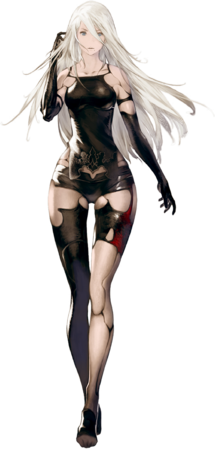
\includegraphics[width=0.49\textwidth,height=17cm]{Nier/Chara/YoRHa_No-2A.png}}
	\caption{Wichtige Nebencharaktere} 
\end{figure}




